% !TeX spellcheck = en_GB
\documentclass[11pt,fleqn]{article}

\usepackage{SpeedyGonzales}
\usepackage{MediocreMike}
\usepackage{Blastoise}

\title{Feature Extraction and Visualization}
\author{Asger Schultz, Rasmus Bryld, and William Marstrand\\
	s183912, s183898, and s183921}
\date{\today}

\pagestyle{fancy}
\fancyhf{}
\lhead{Technical University of Denmark \\
	Asger Schultz, Rasmus Bryld, William Marstrand}
\chead{}
\rhead{Course: 02450}
\rfoot{Side \thepage{} af \pageref{LastPage}}

\graphicspath{{Billeder/}}
\linespread{1}
\geometry{top=2cm, bottom=2cm}

\newcommand{\respdist}[3]{
	\vspace*{-.5cm}
	\begin{table}[H]
	\small
		\begin{tabular}{l r}
			\multicolumn{2}{l}{\textbf{Responsibility distribution}}	\\
			Asger Schultz&	#1\pro\\
			Rasmus Bryld&	#2\pro\\
			William Marstrand&#3\pro
		\end{tabular}
	\end{table}
	\vspace*{-.3cm}
}


%\numberwithin{equation}{section}
\numberwithin{footnote}{section}
\numberwithin{figure}{section}
\numberwithin{table}{section}

\begin{document}
\maketitle
\begin{figure}[H]
	\centering
	
\includegraphics[width=(\textwidth/2)]{DTU_logo}
\end{figure}
\thispagestyle{empty}
\clearpage
\tableofcontents
\vspace{2cm}
\paragraph{Notes on code and data} All source code files will be included along with the report. The full project, including data, is freely available at \url{https://gitlab.gbar.dtu.dk/s183912/skynet}. The data can also be fetched from \url{www.noegletal.dk} by downloading all available data as a \code{.csv} file. However, we recommend getting the data from the file \code{src/full\_noegletal.csv}, partially to ensure the data is the same, and partially to prevent encoding issues, as the \code{.csv} file from \url{www.noegletal.dk} is not \code{utf-8} encoded.

\clearpage

\section{Dataset and methods}
\respdist{20}{30}{50}
The dataset is acquired  from \url{http://noegletal.dk} provided by the Danish Ministry of Social Affairs and the Interior. It regards key figure measurements of demographic, economical, and social data related to the municipalities of Denmark i.e. number of inhabitants, expenses on education, reported burglaries per 1000 inhabitants, etc.
The data for each attribute has been recorded such that they are comparable between the municipalities.
\\
The dataset is generally considered to be of good quality, as it stems from various public censuses, figures, and registers, that are being maintained continuously.
However, there is one noteworthy issue when working with the full dataset: Due to the municipality reform of 2007, the number of municipalities dropped significantly in 2007, and most boundaries changed.
This means that observations from before 2007 are estimated differently than before 2007, as they are based on the former municipalities.
Also, observations from this year (2019) have a great amount of missing values. 
To avoid these issues, this projects only uses data from 2007 until 2018.
\\
This project is focused on using a subset of the key figure measurements to create an understanding of the dataset, and for detecting relationships between figures, that might help spark ideas for areas to investigate in the municipalities.

\subsection{Attributes}
\respdist{50}{30}{20}
The complete dataset contains 180 attributes for every year since 1993.
One of these attributes, however, contains no data, so 179 attributes are left.
Among these there are 473634 possible observations, of which roughly 26\pro\ are missing.
The missing values are mainly due to certain figures either being periodical, e.g. election statistics, or being geographically limited.
Removing all attributes with even a single missing value leaves 49 attributes covering a total of 129654 observations.\\
\\
The attributes are a mixture of discrete and continuous.
For instance, the number of citizens in a given year is discrete, whereas the share of these aged 0-2 is continuous.
The dataset contains no strictly nominal, ordinal, or interval types of attributes.
All attributes can be considered to be of the highest order, the ratio type, as it will make sense to use multiplication and division on the observations.\\
In this report we have used abbreviations for the attributes, but the list of chosen attributes with their full names can be found in appendix \ref{app:attrs}.

\subsection{Machine Learning Goals}
\respdist{40}{20}{40}
Based on the two following reports for this course our primary goals from working with the dataset regards a regression problem for supervised learning and a clustering problem for unsupervised learning.

\subsubsection{Regression Problem - Thefts and Burglaries X Years in the Future}
We will first use regression to try and predict how the number of thefts and burglaries will be a given number of years in the future.
To do this, we need to select attributes that are likely to be indicative of the change in burglaries.
For this report, we chose attributes based on what we expect to be relevant from on our own understanding of society, i.e. we expect high property value to be correlated with burglaries. 
Other ways of selecting attributes may be to explore, choosing the attributes most correlated to the target attribute, or, if practical, using every attribute, but for this project we deemed nine attributes as the most important ones.
Examples of the attributes are \textit{reported thefts/burglaries per 1000 inhabitants} (AT), \textit{the share of 25-64 year-olds without vocational education} (EU), and \textit{property values per inhabitant} (GV).
The full list of chosen attributes is available in Appendix \ref{app:attrs}.
We expect having to standardize data by subtracting the mean and dividing by the standard deviation to prevent observations of different scales causing issues.

\subsubsection{Clustering Problem - Grouping of Municipality Types}
Secondly we will try to use clustering, for instance K-nearest neighbours, to try grouping Municipalities together into to types.
We hope the grouping, if successful, might help reveal if different types of municipalities are more susceptible to theft and burglaries than others.

\subsection{Summary statistics}
\respdist{10}{80}{10}
The summary statistics listed in the following were calculated using the Python Data Analysis Library, Pandas, and provides key properties of the data.
\begin{table}[H]
	\centering
	\begin{tabular}{|l|r|r|r|r|r|r|r|r|r|}
		\hline
		& \jls{AT}     & \jls{GV}     & \jls{BG}     & \jls{DT}      & \jls{EU}    & \jls{VU}    & \jls{FO}    & \jls{IV}     & \jls{ATK}   \\ \hline
		count & 1176   & 1176   & 1176   & 1176    & 1176  & 1176  & 1176  & 1176   & 1176  \\ \hline
		mean  & 48.19  & 170091 & 162698 & 6989    & 22.4  & 24.77 & 8218  & 311    & 1663  \\ \hline
		std   & 20.1   & 72358  & 30982  & 1704    & 5.45  & 9.111 & 1074  & 192.4  & 907.4 \\ \hline
		min   & 3      & 77854  & 127232 & 3114    & 8     & 12.7  & 4703  & 15     & -381  \\ \hline
		25\pro\   & 33.475 & 120590 & 144787 & 5652    & 19.3  & 18.8  & 7623  & 188    & 957.5 \\ \hline
		50\pro\   & 46.4   & 145365 & 151852 & 6689    & 23.2  & 22.1  & 8168  & 272    & 1534  \\ \hline
		75\pro\   & 59.225 & 200090 & 169741 & 8320.75 & 26    & 27.3  & 8822  & 363.75 & 2279  \\ \hline
		max   & 140.3  & 470129 & 337689 & 12597   & 38.70 & 59.3  & 11904 & 1368   & 4964  \\ \hline
	\end{tabular}
\end{table}\noindent
For each attribute, a box plot was made, all of which can be seen on figure \ref{fig:bp}. As the summary table suggests, the observations of the different attributes are distributed quite differently, which will be explored further in the next chapter.

\section{Data Visualization}
\respdist{50}{20}{30}
\subsection{Outliers and Distribution}
To inspect the distribution of the data, quantile-quantile plots (QQ-plots) were constructed.
In these, theoretical quantiles from a normal distribution are plotted against the observations.
If there is a strong, linear correlation, the data can be said to be normally distributed.
This was done for all selected attributes.
The plots can be seen in figure \ref{fig:qq}.
The QQ-plots show that some variables are close to normally distributed, such as gross daycare expenses per inhabitant, whereas others, such as property values per inhabitant, are far from it.\\
\\
The box plots show that a fair number of outliers.
However, these are quite numerous and for the most part not clustered, so it is not considered a significant issue.
The QQ plots also allow further probing for outliers, as the observed values are shown on the $y$-axis.
Apart from six observations (out of 2646) in job activation expenses, there are no significant outliers, and even these six are not by any means extreme.
Therefore, outliers are not deemed a major issue.

\subsection{Correlations}
The correlation between two vectors of length $ N $ $ \mathbf x\andim\mathbf y $ is given as
\begin{equation*}
	\operatorname{corr}(x, y)=\frac{1}{N-1}\frac{\sum_{i=1}^{N}(x_i-\mu_{\mathbf x})(y_i-\mu_{\mathbf y})}{\operatorname{std}x\operatorname{std}y}
\end{equation*}
Calculating the correlation matrix for all attributes in Appendix \ref{app:attrs} such the $ (i, j) $'th entry is the correlation between the $ i $'th and $ j $'th variable in the list in the appendix, the correlation matrix becomes
\begin{equation*}
	\mathbf \Sigma=\begin{bmatrix}
		1.00	&	0.22	&	0.35	&	0.60	&	-0.24	&	0.35	&	0.10	&	0.55	&	-0.19\\
		0.22	&	1.00	&	0.87	&	0.38	&	-0.65	&	0.64	&	0.24	&	0.15	&	-0.12\\
		0.35	&	0.87	&	1.00	&	0.53	&	-0.77	&	0.80	&	0.19	&	0.19	&	-0.18\\
		0.60	&	0.38	&	0.53	&	1.00	&	-0.52	&	0.48	&	0.44	&	0.58	&	-0.19\\
		-0.24	&	-0.65	&	-0.77	&	-0.52	&	1.00	&	-0.90	&	0.02	&	-0.05	&	0.08\\
		0.35	&	0.64	&	0.80	&	0.48	&	-0.90	&	1.00	&	-0.09	&	0.17	&	-0.08\\
		0.10	&	0.24	&	0.19	&	0.44	&	0.02	&	-0.09	&	1.00	&	0.31	&	-0.29\\
		0.55	&	0.15	&	0.19	&	0.58	&	-0.05	&	0.17	&	0.31	&	1.00	&	0.21\\
		-0.19	&	-0.12	&	-0.18	&	-0.19	&	0.08	&	-0.08	&	-0.29	&	0.21	&	1.00
	\end{bmatrix}
\end{equation*}
As the final goal is to predict how thefts and burglaries (AT) will change in the future, the correlation was calculated such that the correlations between AT and other attributes were actually the correlation between the given attribute and AT five years later.\\
\\
Most attributes are rather weakly correlated, though some, like property values (GV) and taxable amount (BG), are fairly strongly correlated. In the following figure, a few of the attributes are plotted against AT five years later.
\begin{figure}[H]
	\centering
	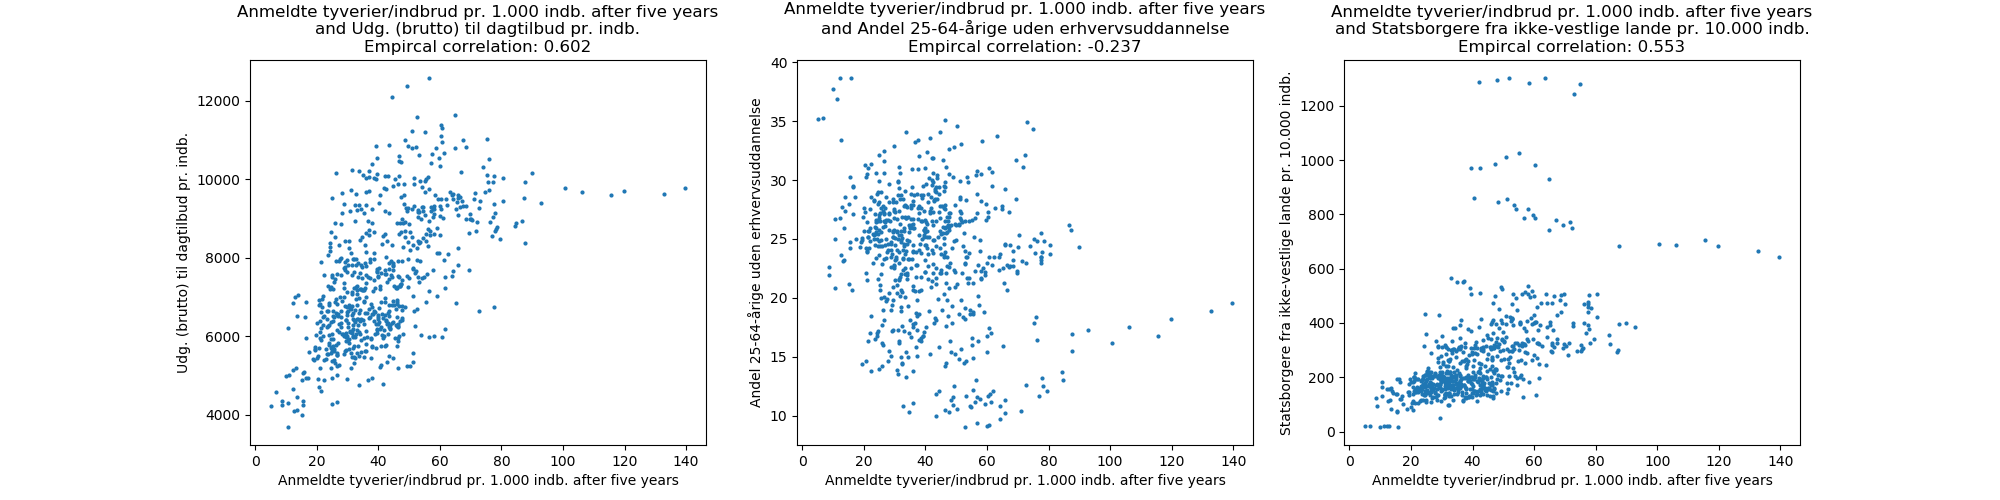
\includegraphics[width=1\textwidth]{corrs}
\end{figure}\noindent
As previously indicated by the correlations, none of plotted attributes are strong indicators of how AT will look five years into the future, though there are some fairly weak trends.

\subsection{Feasibility}
Based on the correlations and plots, the primary modelling goal does not seem easily achievable.
However, the correlations alone do not tell the full story.
Thefts and burglaries may be more strongly connected to some combinations of features that would not be revealed by the correlation analysis. A more sophisticated machine model, such as a neural network, may well be able to model such connections.
It is also worth mentioning that we have only looked into the relation between AT and eight other features here, but that there are a 170 other features, some of which may more indicative of the change in thefts and burglaries.
The problem could also be simplified to only try predict thefts and burglaries up to for instance two years into the feature.\\
\\
So, while this preliminary analysis is not promising, there are good reasons to believe that the end goal is possible.
\pagebreak

\section{Principal Component Analysis}
\respdist{20}{20}{60}
We have investigated our data and the attributes we have chosen.
Another interesting question now becomes if we can represent our data in a more compact way.
Specifically we are interested in using Principal Component Analysis (PCA) to reduce the dimensionality of our data and investigate how each of the attributes affects the variation of our dataset.\\
Before carrying out PCA, all attributes were standardized by subtracting the mean and dividing by the empirical standard deviation, as the different attributes varied quite significantly in scale, which can have big impacts on PCA.
\\
Having done PCA, we first look at a scatter plot of the Municipality Key Figure Data when it has been projected into the PCA subspace of principal component 1 and 2.
\begin{figure}[H]
	\centering
	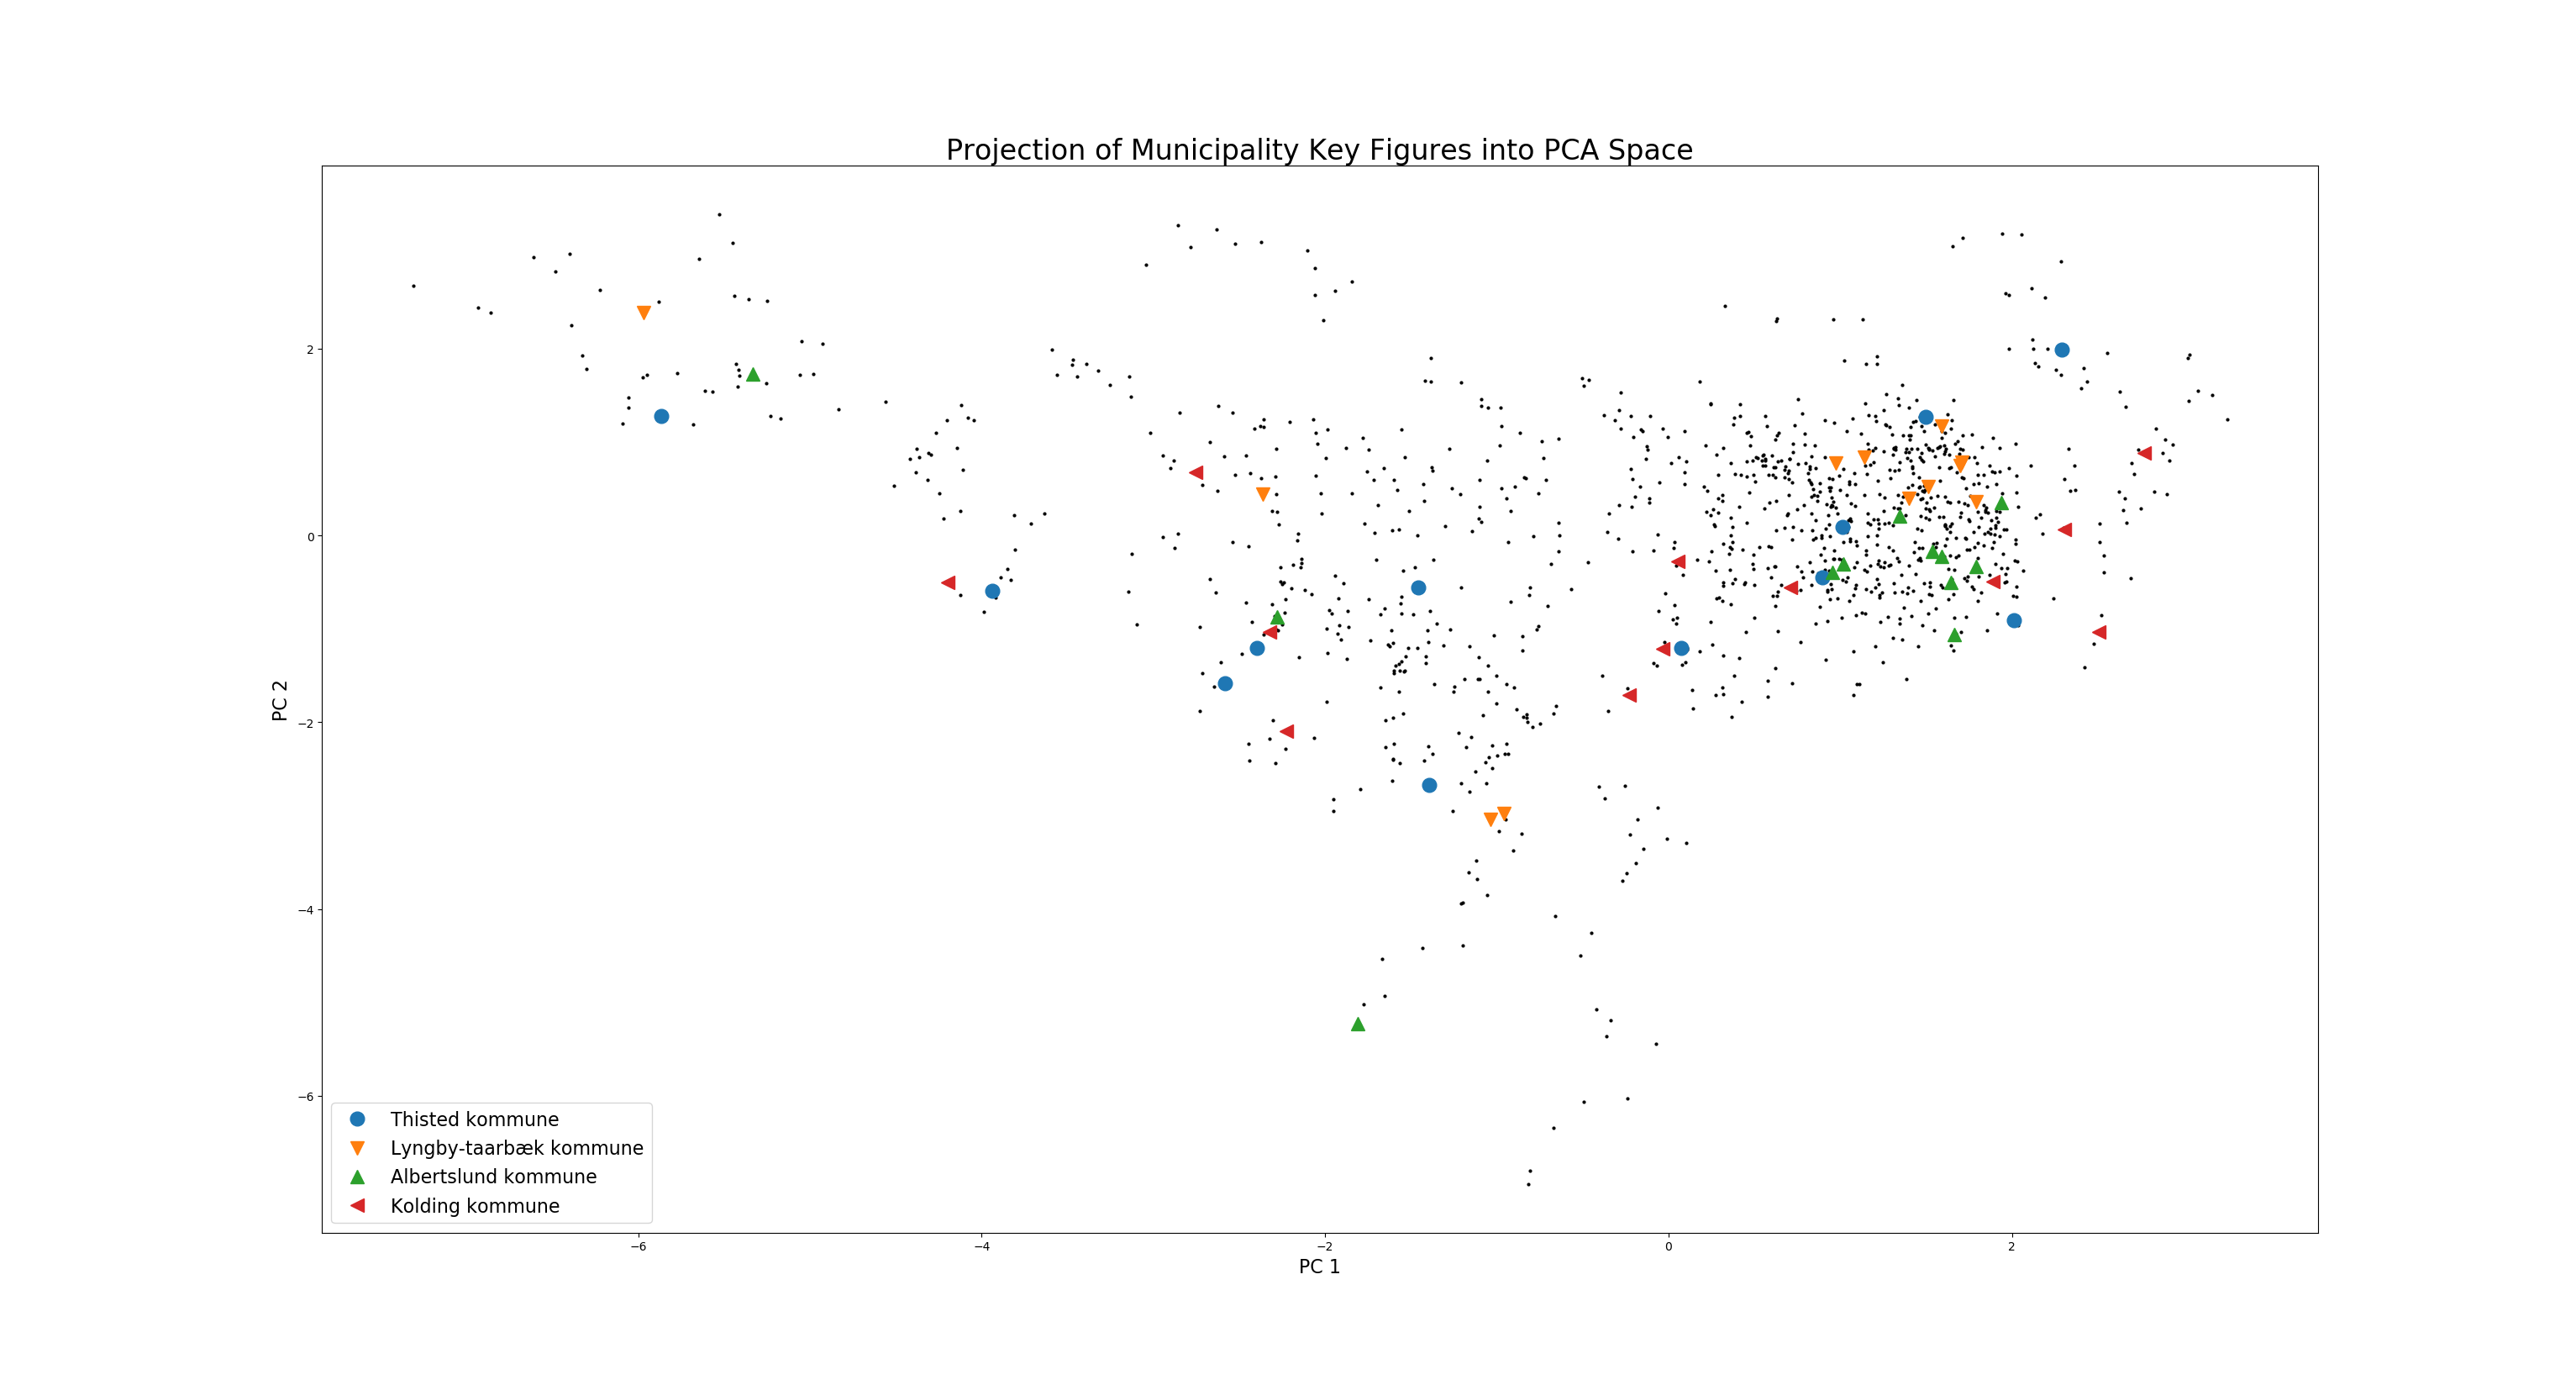
\includegraphics[width=\textwidth]{PCA_scatter}
	\caption{Scatter Plot for Projection of Data into PCA Space}
	\label{scatter}
\end{figure}\noindent
When we look at the plot in figure \ref{scatter} we can see the greatest spread along principal component 1 (PC1) and the second most along the PC2 axis. This fit with the theoretical expectations of PC1 having the greatest variance.\\
The scatter plot has four cities highlighted with different markers. In the plot we see a large spread for Thisted, and Kolding along PC1 while Albertslund and Lyngby-taarbæk are clustered more to the right. Still, it is difficult to divide the data points for each municipality into groups.\\
This could indicate that the attributes we have chosen to look at might not be relevant for clustering of the municipalities. Another reason could be that PC1 and PC2 do not explain enough variance to provide a useful grouping of the data points.\\
To investigate this, we will create a plot for the variance explained by our principal components.
\\
To take a closer look at how much of the variance is actually explained by each principal component we can use the following plot
\begin{figure}[H]
	\centering
	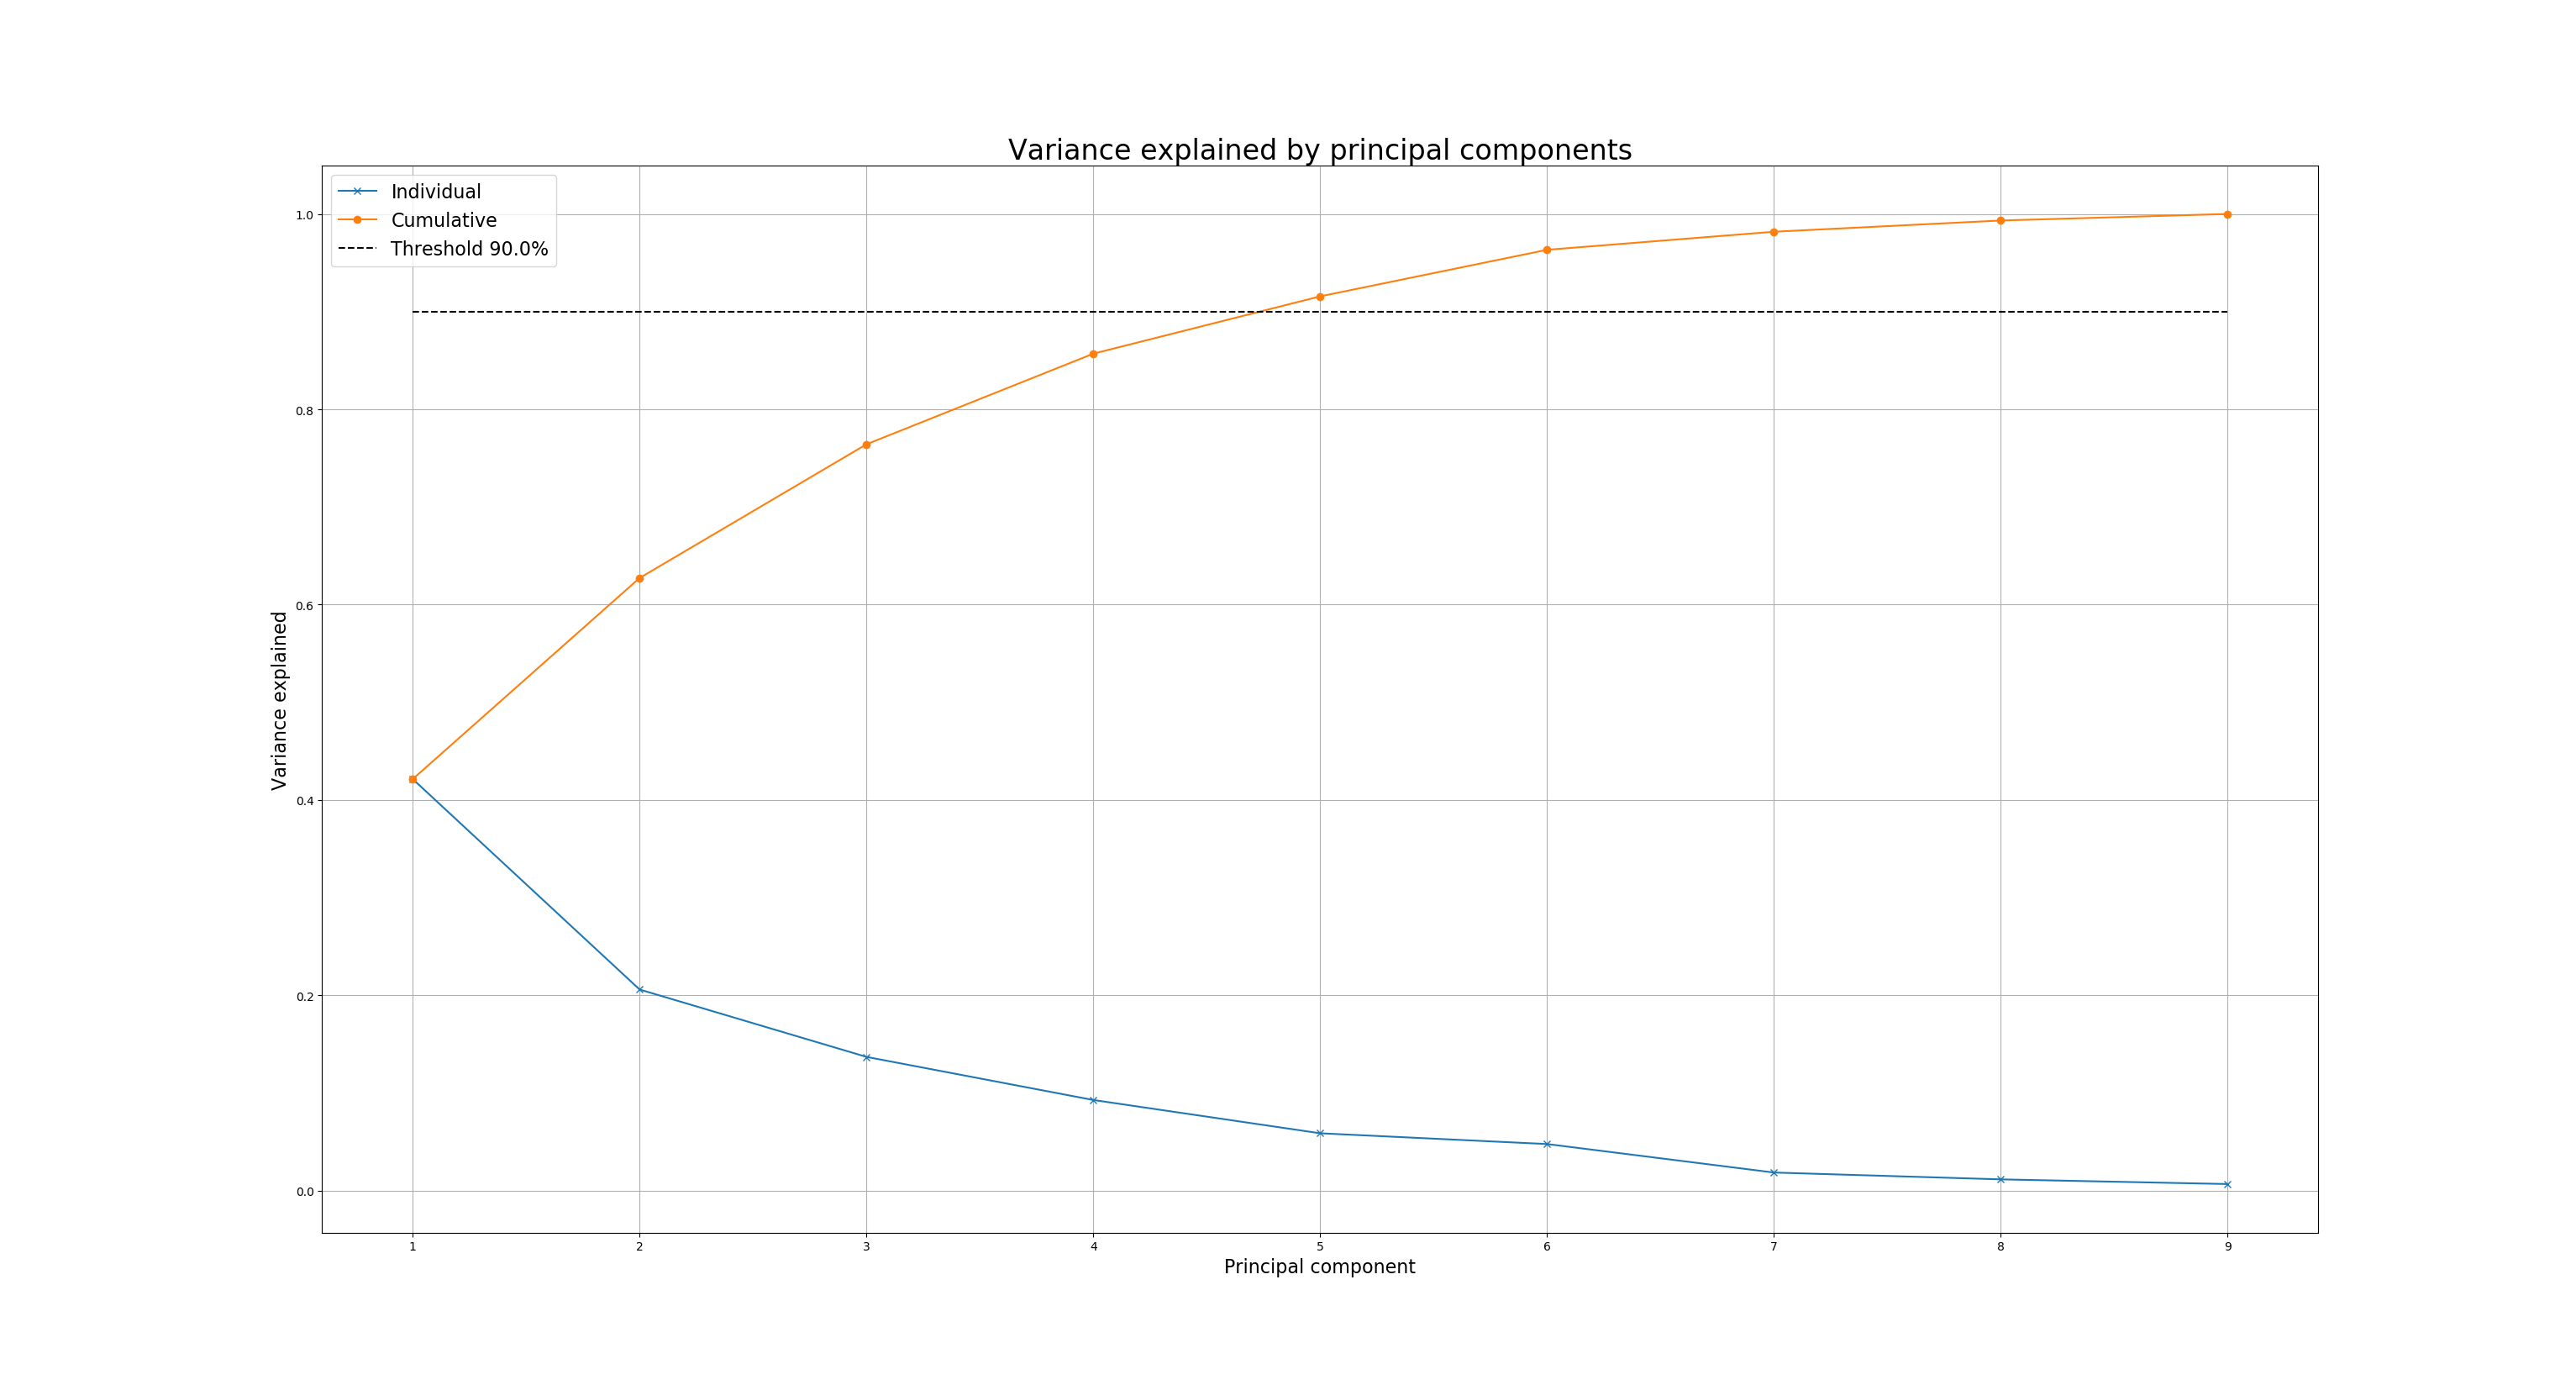
\includegraphics[width=\textwidth]{variance_explained}
	\caption{Individual and Cumulative Variance explained by the Principal Components}
	\label{var_explain}
\end{figure}\noindent
From figure \ref{var_explain} we see, that PC1 holds around twice as much variance as PC2, which fits with the larger spread across the PC1-axis in the scatter plot of figure \ref{scatter}.
And we see that to get more than 90\pro\ of the variance in our data, we have to use at least five principal components. This might also explain why it was difficult to group data in figure \ref{scatter} using only PC1 and PC2.
\\
This knowledge is useful, if we for instance want to compress our data, while still keeping enough variance to be able to explain it again afterwards.
Now we know how many principal components we need to keep at least 90\pro\ of the variance in our data, but it would also be interesting to go a bit deeper and look at the attributes of our principal components.
\\
For instance, we could look at the coefficients related to each attribute in the first five principal components to get insights on how the attributes create the variance.
\\
\begin{figure}[H]
	\centering
	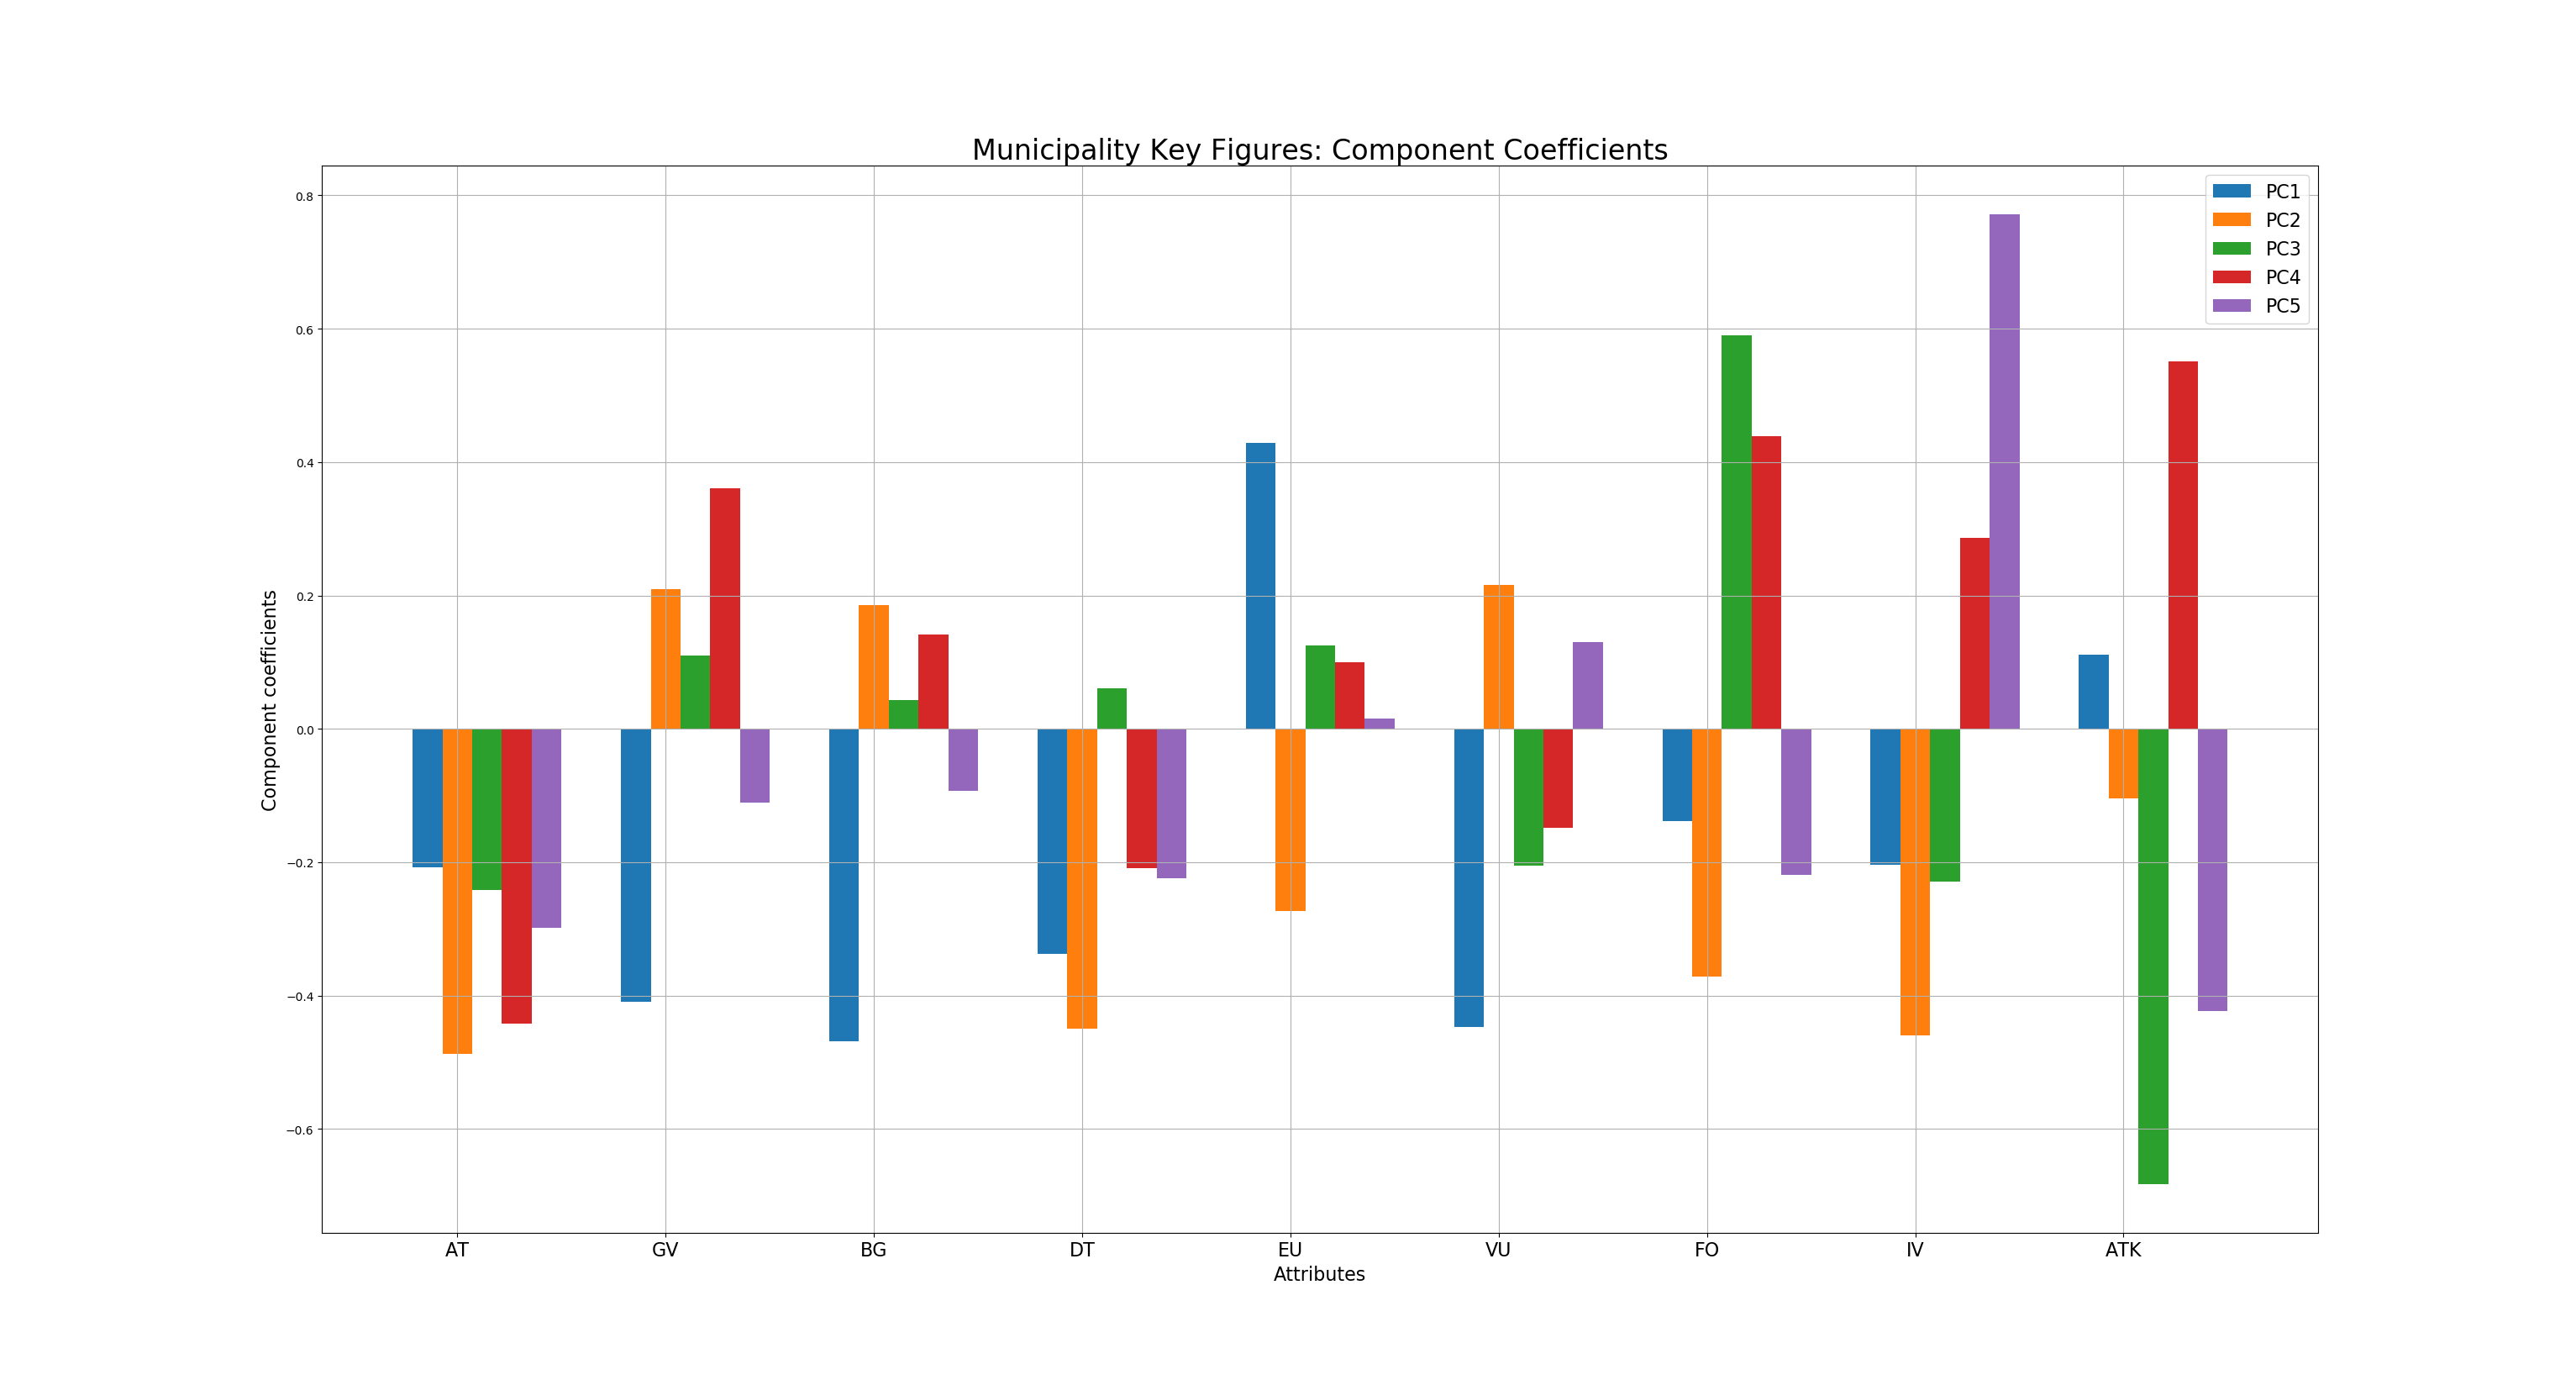
\includegraphics[width=\textwidth]{component_coefficients}
	\caption{Attribute Coefficient Values of the first five PCs}
	\label{att_coef}
\end{figure}\noindent
We can for instance use figure \ref{att_coef} to see what attributes are important for the variance of the different principal components.
If we look at PC1, we see that large variance is found between large negative values of AT, BG, DT, VU, and a large positive value of EU, while ATK, and FO are not that relevant.\\
If we now were to include PC3, PC4, and PC5, figure \ref{att_coef} tells us, that for PC3, and PC4 FO, and ATK might be more useful, while for PC5 attributes ATK and IV might be more relevant for the data variance.\\
Also, by doing these investigations for the different PCs we can get a feeling of what \textit{combinations} of attributes creates the greatest spread in our data.
For instance taking PC1 as the current example.
If we have some new data and we project it into our current PCA space.
If the data has large negative values for GV, BG, DT, VU and large positive values for EU it will get large positive values from the projection onto PC1.
If the opposite is true and GV, BG, DT, and VU are positive and EU is negative, then the data gets large negative values from the projection onto PC1.
So for the scatter plot in figure \ref{scatter} this would mean either going far to the left or far to the right.
\\
We can illustrate this idea of the attributes moving in different directions depending of their coefficients in the different principal component subspaces.
If we again look at PC1 and PC2 and their attribute coefficients as vectors we can make the following plot
\begin{figure}[H]
	\centering
	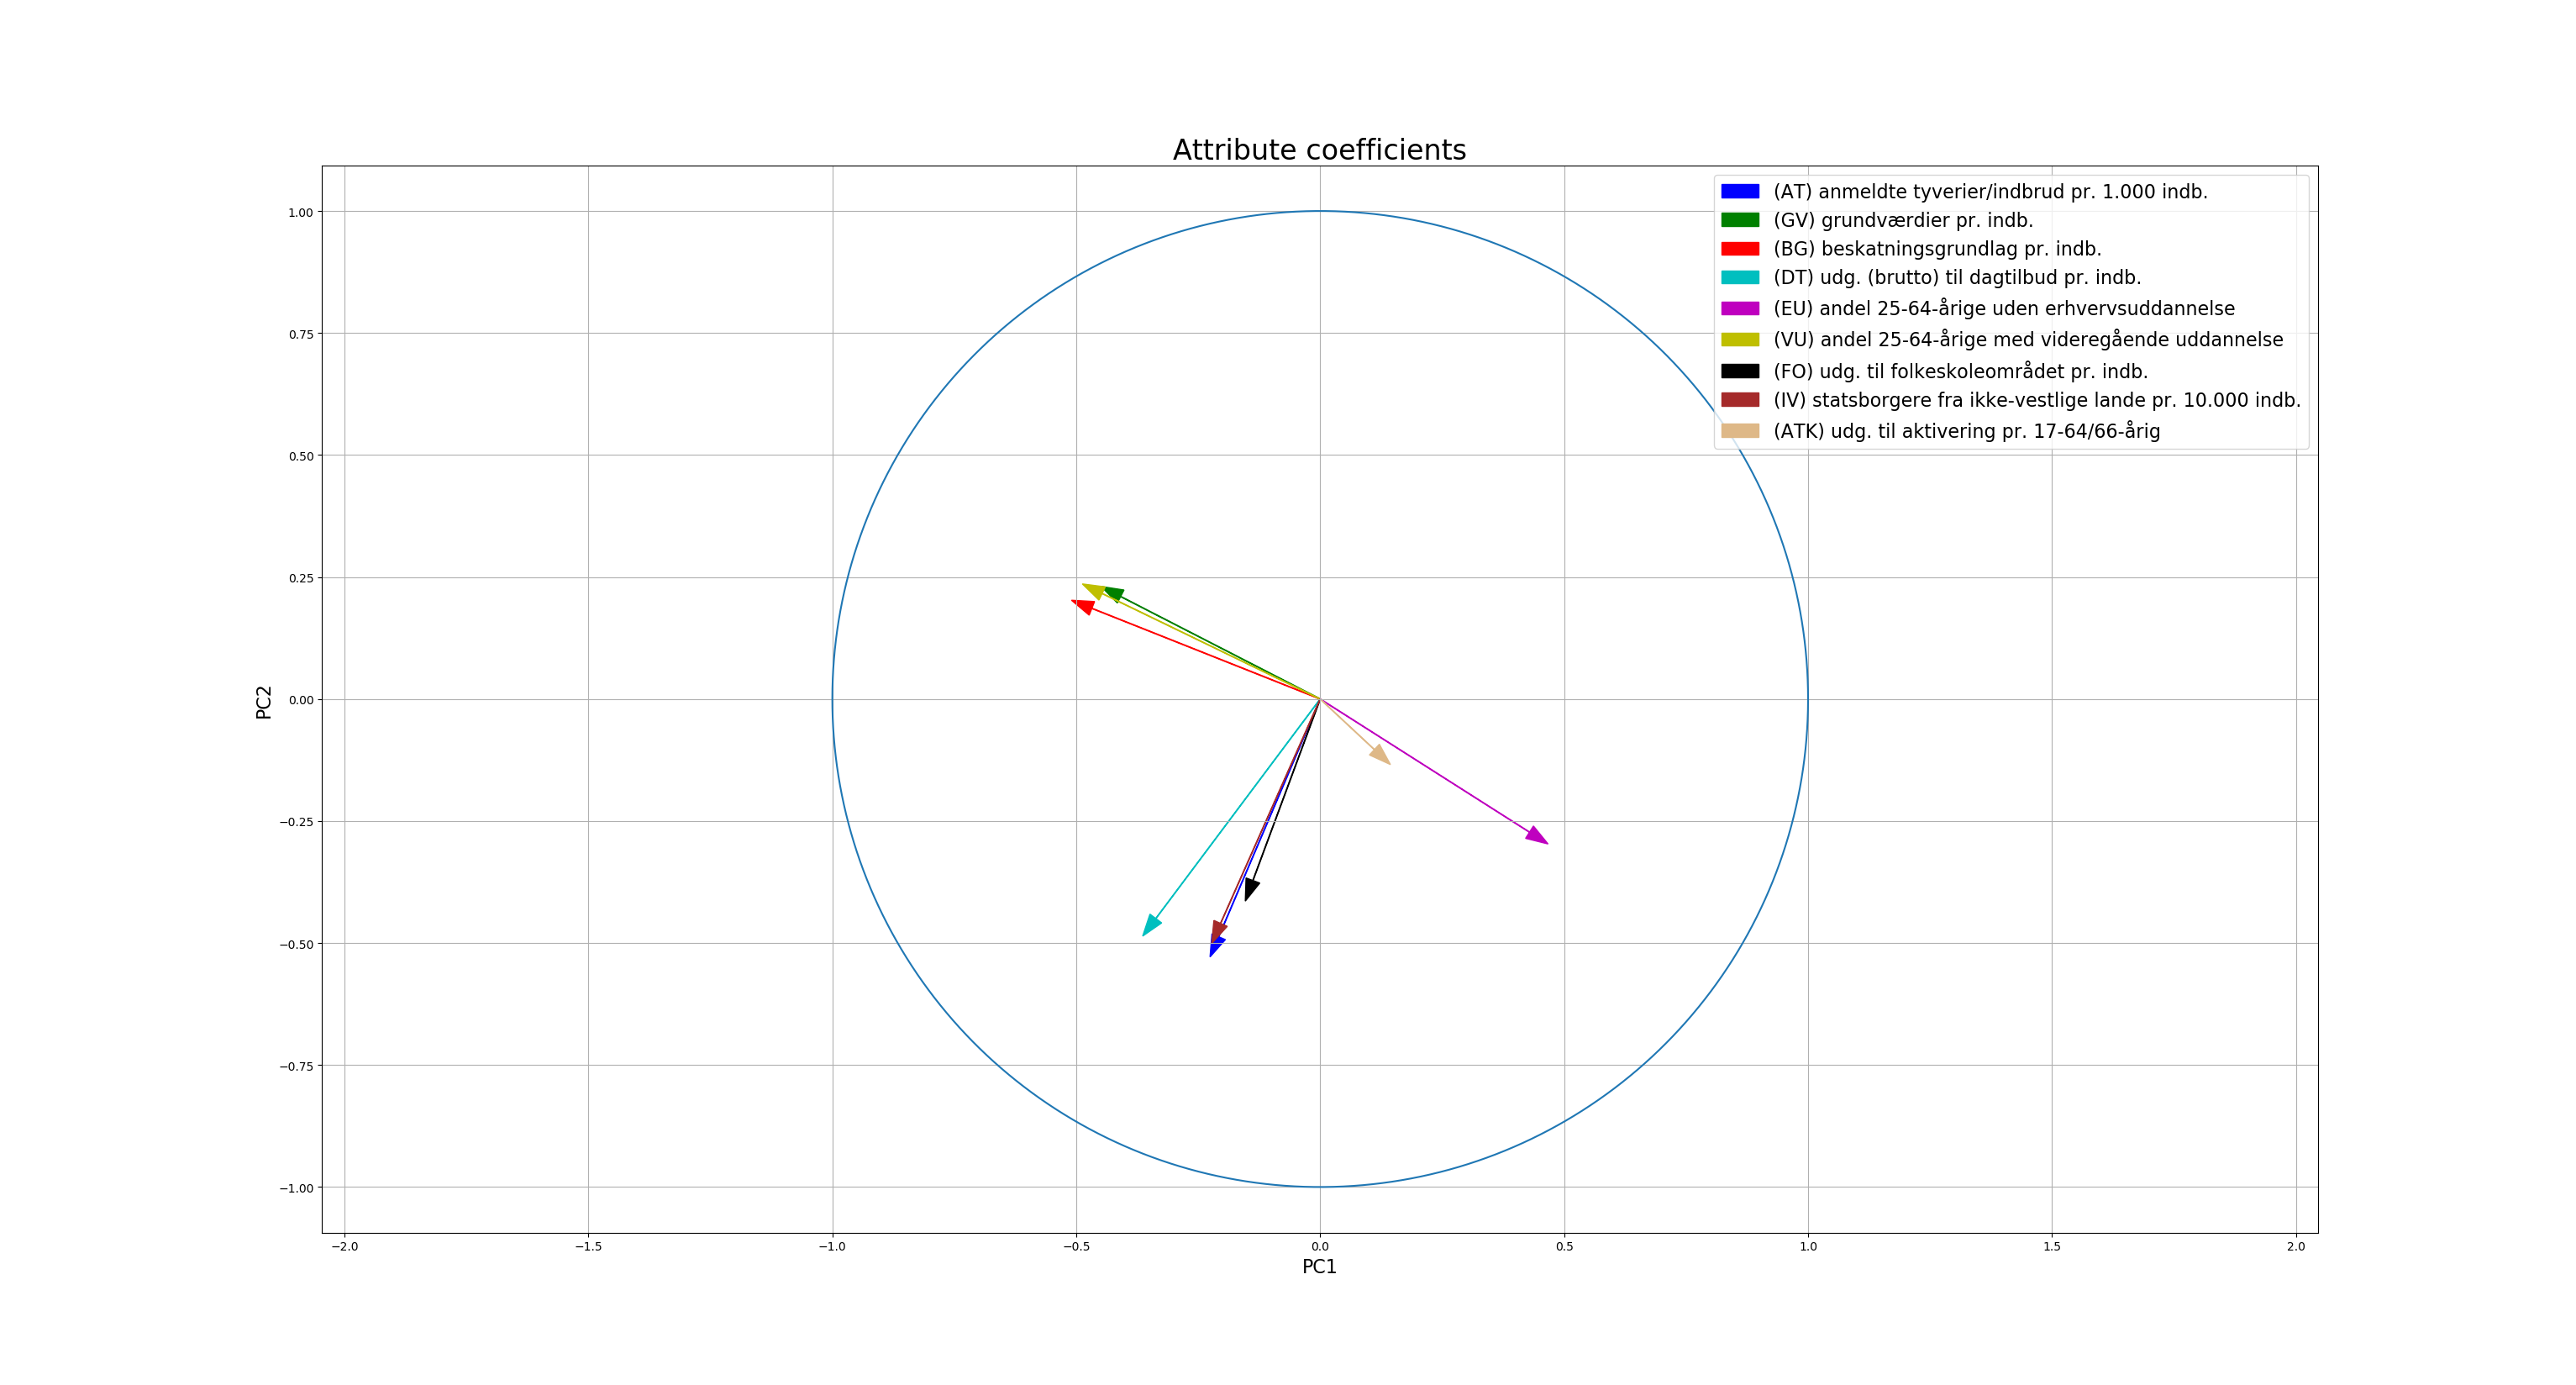
\includegraphics[width=\textwidth]{attribute_coefficients_arrows}
	\caption{Vector Visualization of Attribute Coefficients}
	\label{att_vec}
\end{figure}\noindent
Figure \ref{att_vec} shows the directions each of the attributes are "pulling" in the PC1/PC2 subspace and how much they pull (length of the vectors).
This can also give us an intuition on how data will behave when projected into the PC1/PC2 subspace.
For instance if we have data with high EU and high GV, and low values on the other features.
Then the projection will be around zero, because EU and GV will pull in opposite directions and with approximate the same "force".
\\\\
This concludes our PCA investigation.
The investigation has shown us, that we need at least five of our nine principal components to explain our desired 90\pro\ of the variance in the data.
Also, it has shown us, that if we want to distinguish between municipalities from our data, then a big variation can be found between municipalities on specific attribute values.
\clearpage
\section{Discussion}
\respdist{40}{30}{30}
From our analysis of the data, we learned that the data in general is of good quality with some exceptions.
There are few missing values and outliers.
The distribution of the nine observations we investigated vary quite significantly, with some being normally distributed and some not.
Using Principal Component Analysis, we found it was possible to explain over 90\pro\ of the total variance using five principal components, a significant reduction of the nine dimensions of the data.
Our machine learning modelling goal of predicting the development of thefts and crime into the future appears doable, though not necessarily straightforward.
Based on the PCA, clustering also appears doable.
It is important to note that we only looked at a fairly small amount of the available data, and so an important step in the coming machine learning modelling will be to include more data and use more rigorous methods of selecting useful attributes than qualified guesses. Decreasing the complexity of the regression task to only predict a few years into the future should also help.
All in all, we are optimistic that both modelling tasks are well within the realm of possibility.

\clearpage


%TODO
\begin{thebibliography}{9}
	\item Ministry of Social Affairs and the Interior: "SIM's Municipal Key Figures". At: \url{http://noegletal.dk}. Visited sep $19^{\text{th}}$, 2019. (Webpage, in Danish)
	\item University of Virginia: "Understanding Q-Q plots". At: \url{https://data.library.virginia.edu/understanding-q-q-plots/}. Visited sep $20^{\text {th}}$, 2019. (Webpage)
\end{thebibliography}

\appendix
\section{Chosen attributes}\label{app:attrs}
For this report we selected the following attributes to investigate:
\begin{itemize}
	\item[-] (AT) Anmeldte tyverier/indbrud pr. 1.000 indb. (Reported thefts/burglaries per 1,000 inhabitants)
	\item[-] (GV) Grundværdier pr. indb. (Property values per inhabitant)
	\item[-] (BG) Beskatningsgrundlag pr. indb. (Taxable amount per inhabitant)
	\item[-] (DT) Udg. (brutto) til dagtilbud pr. indb. (Gross daycare expenses per inhabitant)
	\item[-] (EU) Andel 25-64-årige uden erhvervsuddannelse (Share of 25-64 year-olds without vocational education)
	\item[-] (VU) Andel 25-64-årige med videregående uddannelse (Share of 25-64 year-olds with tertiary education)
	\item[-] (FO) Udg. til folkeskoleområdet pr. indb. (Expenses towards public primary school per inhabitant)
	\item[-] (IV) Statsborgere fra ikke-vestlige lande pr. 10.000 indb. (Citizens from non-western countries per 10,000 inhabitants)
	\item[-] (AKT) Udg. til aktivering pr. 17-64/66-årig (Expenses towards job activation per 17-64/66 year-old)
\end{itemize}

\section{QQ plots}
\begin{figure}[H]
	\centering
	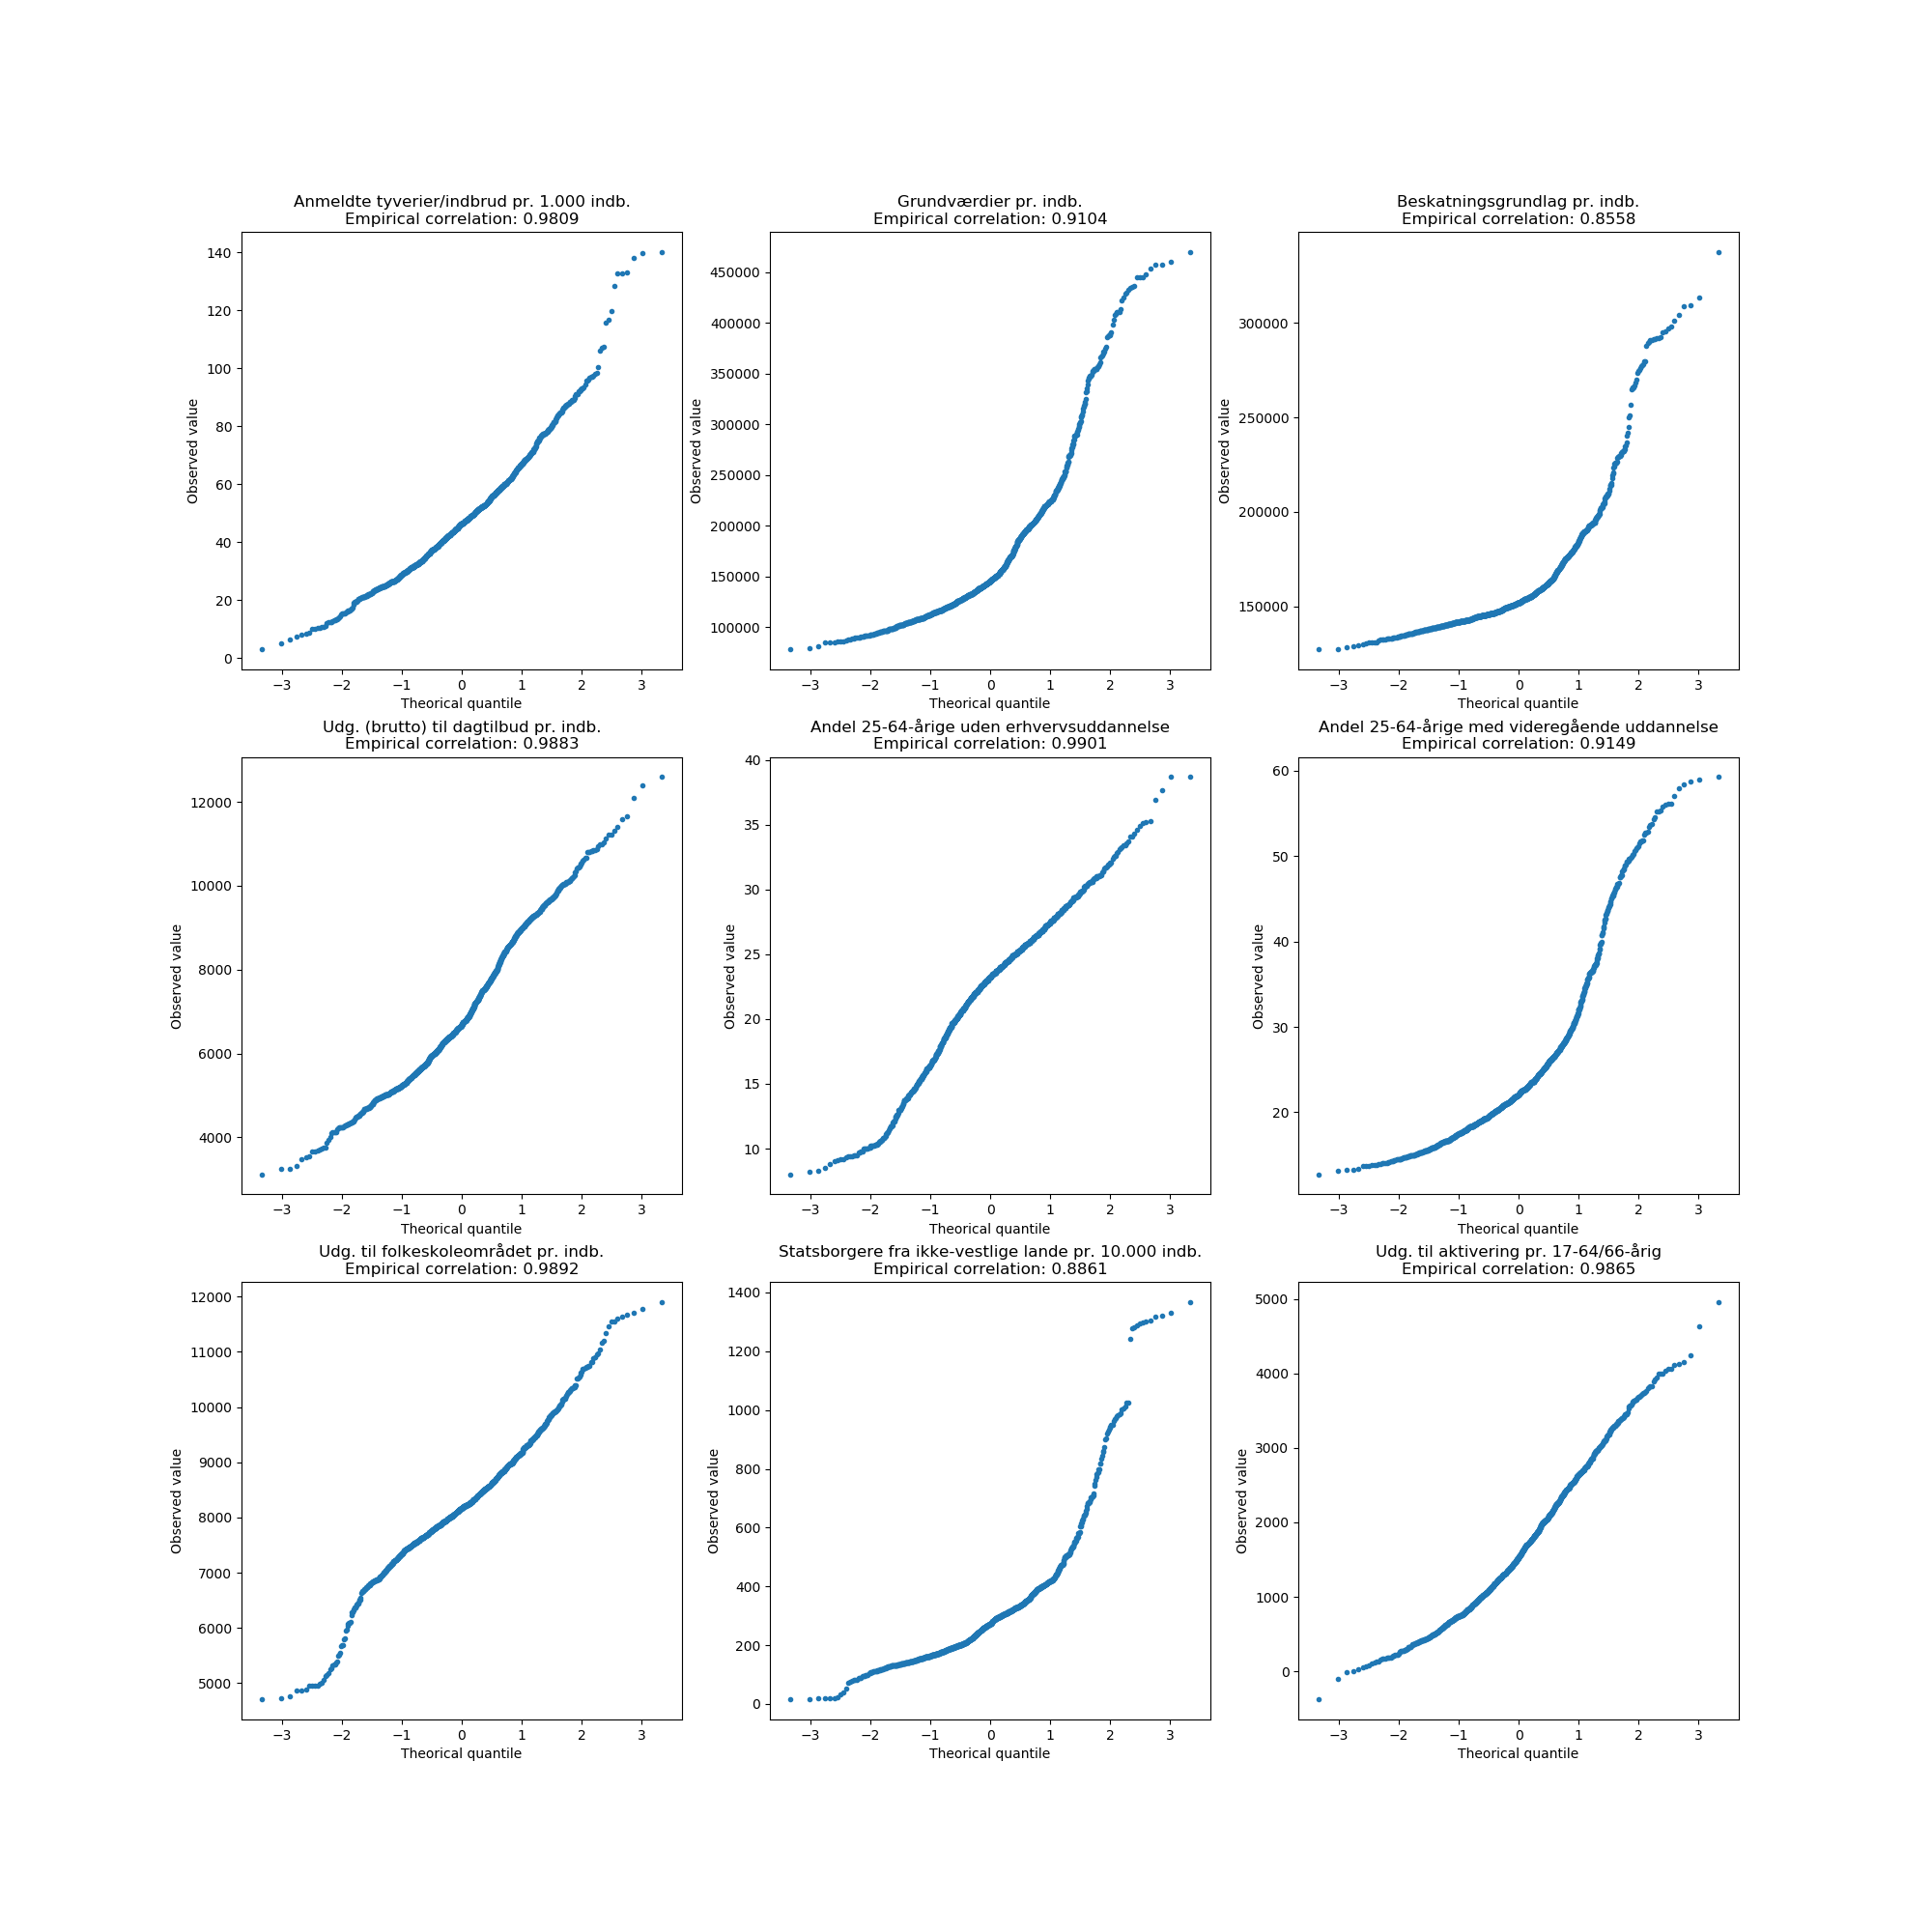
\includegraphics[width=\textwidth]{qq-plots}
	\caption{QQ plots for attributes listed in appendix \ref{app:attrs}.}\label{fig:qq}
\end{figure}
\section{Box plots}
\begin{figure}[H]
	\centering
	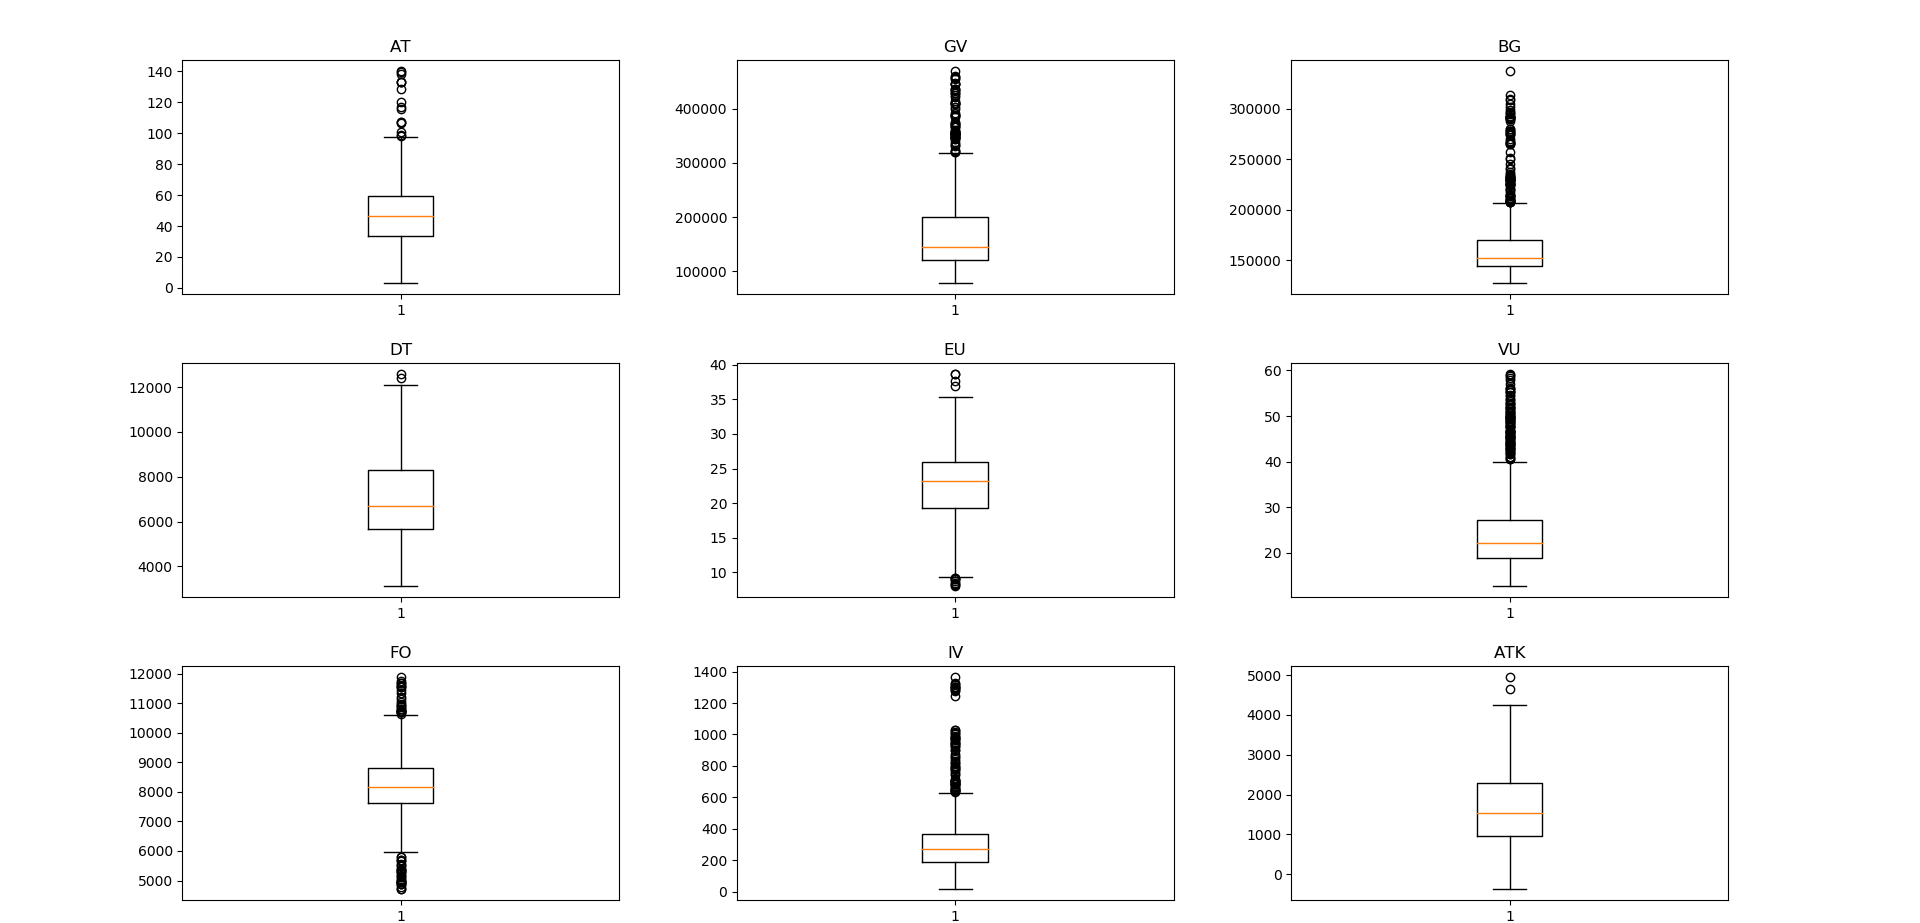
\includegraphics[width=\textwidth]{boxplot_statistics}
	\caption{Box plots for attributes listed in appendix \ref{app:attrs}.}\label{fig:bp}
\end{figure}

\end{document}
